\documentclass[11pt]{article}
\usepackage{amsmath,amsthm,amssymb,amsfonts}
\usepackage{enumerate}
\usepackage{color}
\usepackage[margin=1in, top=.5in]{geometry}
\usepackage{float}
\usepackage[parfill]{parskip}

\usepackage{tikz}
\usetikzlibrary{graphs, graphs.standard,arrows}

\DeclareMathOperator*{\argmin}{arg\,min}
\DeclareMathOperator*{\argmax}{arg\,max}
\DeclareMathOperator*{\adjoint}{ad}

 
\newcommand{\N}{\mathbb{N}}
\newcommand{\Z}{\mathbb{Z}}
\newcommand{\C}{\mathbb{C}}
\newcommand{\Q}{\mathbb{Q}}
\newcommand{\R}{\mathbb{R}}
\newcommand{\norm}[1]{\left\lVert#1\right\rVert}
\newcommand{\SE}[1]{\text{SE(#1)}}

\newcommand{\pose}[2]{{}^{#1}T_{#2}}

\newenvironment{problem}[2][Problem]{\begin{trivlist}
\item[\hskip \labelsep {\bfseries #1}\hskip \labelsep {\bfseries #2.}]}{\end{trivlist}}
%If you want to title your bold things something different just make another thing exactly like this but replace "problem" with the name of the thing you want, like theorem or lemma or whatever

%%This optional package allows you to use TikZ to typeset automata
%\usepackage{tikz}
%\usetikzlibrary{automata}
%
%%This optional package allows you to use xypic to typeset automata
%\usepackage[all]{xy}
%
%%This optional package allows you to include external graphics
\usepackage{graphicx}

%%%%%%%%%%%%%%%%%%%%%%%%%%%%%%%%%%%%%%%%%%%%%%%%%%%%%%%%%%%%%%%%%%%%%%%%%%%%%
%%%%    FILL THESE FIELDS IN
%%%%%%%%%%%%%%%%%%%%%%%%%%%%%%%%%%%%%%%%%%%%%%%%%%%%%%%%%%%%%%%%%%%%%%%%%%%%%

\title{Acrobat Control}
\author{Martin Deegan}
 
\begin{document}
 
\maketitle
\tableofcontents

\section{Lie Groups}

\subsection{Spline trajectory}
We assume to have a time parameterized $C^2$ spline trajectory defined on the \SE{3} manifold. This spline has been created with feasible accelerations and angular rates.
\begin{align}
	X(t)&: \R \to \SE{3}\\
	\dot X(t)&: \R \to \R^6\\
	\ddot X(t)&: \R \to \R^6
\end{align}

\section{Control}

\subsection{Solving for a rotation}
Given a desired force $F_{des}$, we need to find an orientation to apply this force vector. To apply this force, we need to point the normal vector of the plane of the quad in the direction of $F_{des}$. This leaves us one degree of freedom to set: yawing about $F_{des}$. To set the rotation, we find a rotation, $R_{des}$ which points the normal vector towards $F_{des}$ while minimizing the error between $R_{des}$ and the nominal orientation defined by the spline trajectory.

Let $u = F_{des} / \norm{F_{des}}$ be the unit vector in the direction of $F_{des}$. This is also the axis we can rotate about.

\begin{align}
	\texttt{minimize}_{R_{des}}& \frac{1}{2}\norm{\log\left(R(t)^{-1}R_{des}\right)}_2^2\\
	\texttt{subject to }& R_{des}u = u
\end{align}

The constraint fixes the rotations about $F$ (it is an eigenvector of $R_{des}$). Since we are dealing with one degree of freedom, we can reduce this problem to the unconstrained problem.
\begin{align}
\texttt{minimize}_\theta& \frac{1}{2}\norm{\log\left(R(t)^{-1}\exp(\theta u)\right)}_2^2
\end{align}

\begin{figure}[H]
	\centering
	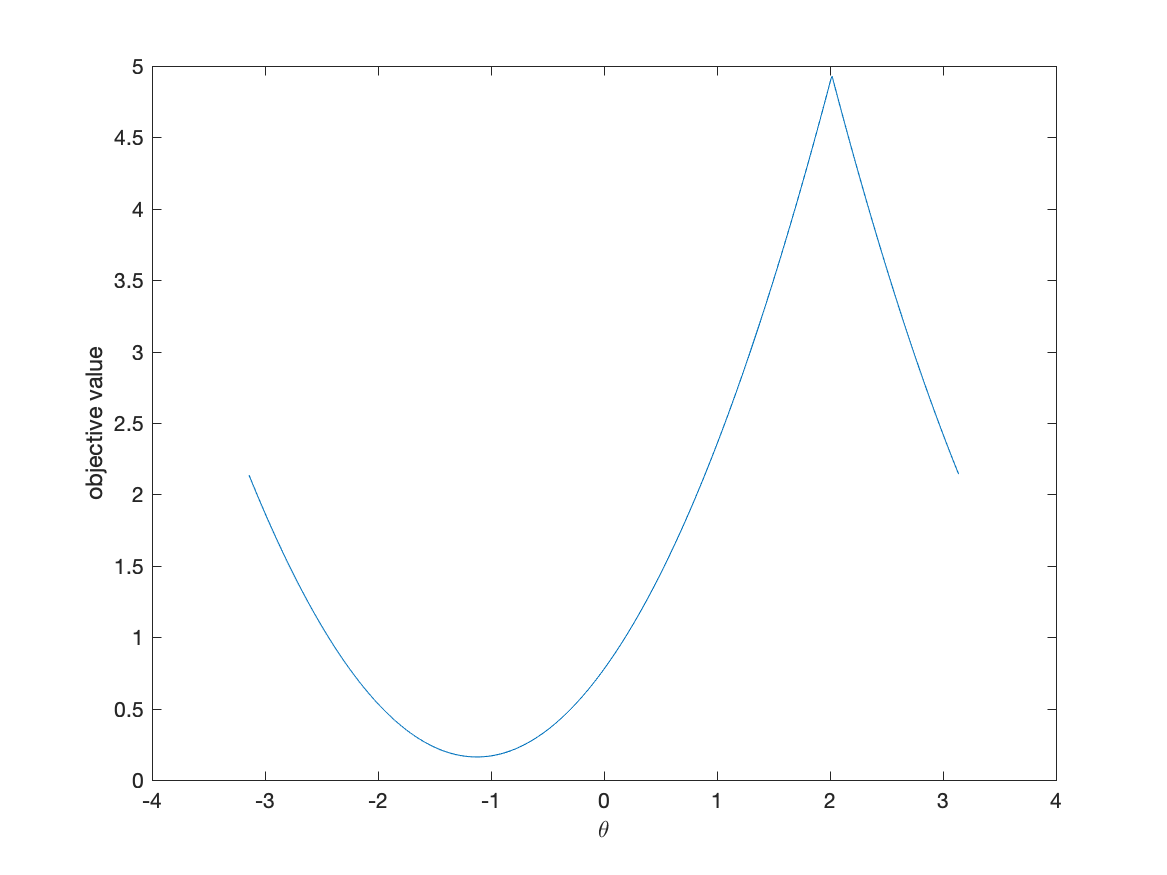
\includegraphics[width=\textwidth]{../matlab/objective_function.png}
	\caption{The value of the objective function for different $\theta \in [-\pi, \pi]$. Clearly non-convex}
\end{figure}

This is non-convex. We can get a convex problem which is close by linearizing. $R(t)^{-1} = \exp(\omega)$.

\begin{align}
\texttt{minimize}_\theta& \frac{1}{2}\norm{\log\left(R(t)^{-1}\exp(\theta u)\right)}_2^2\\
&\approx \frac{1}{2}\norm{\omega + \theta J_r^{-1}(\omega)u}_2^2
\end{align}

\begin{figure}[H]
	\centering
	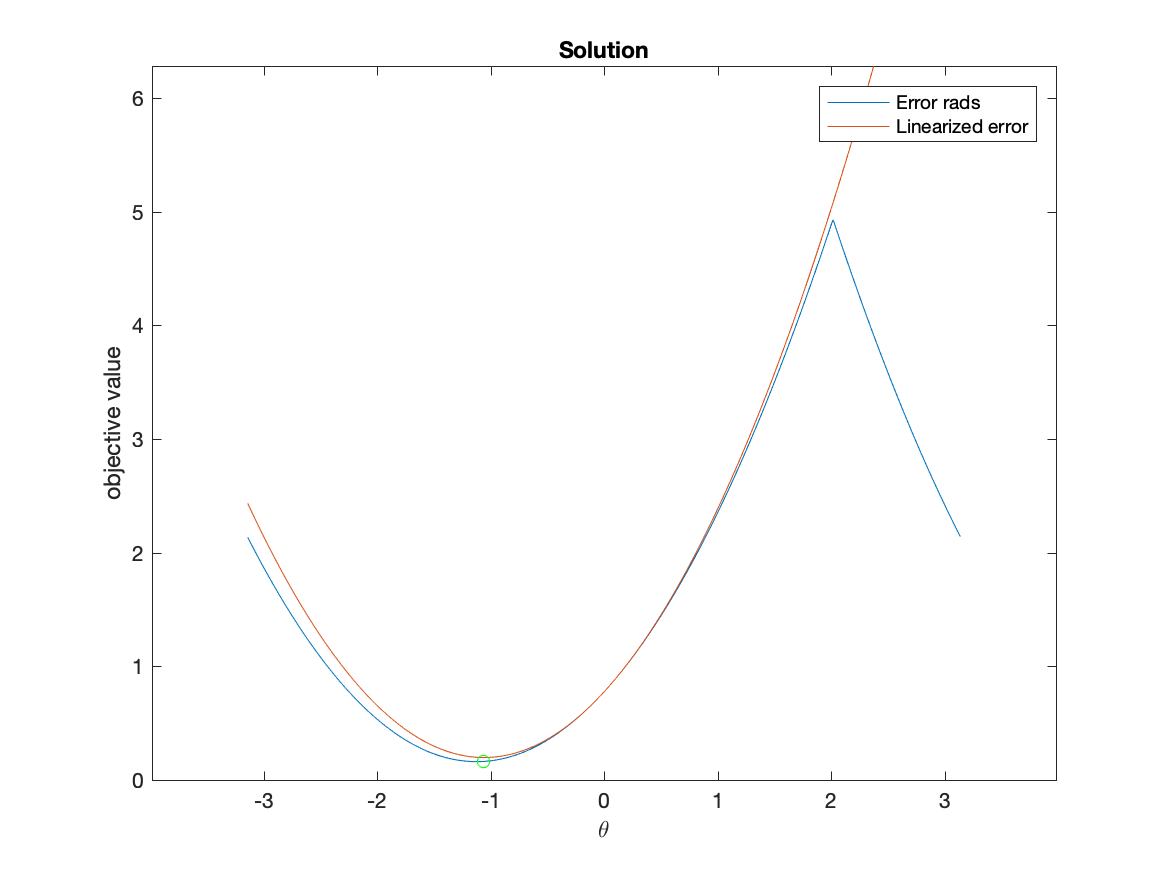
\includegraphics[width=\textwidth]{../matlab/linearized_solution.png}
	\caption{The value of the objective function for different $\theta \in [-\pi, \pi]$ in blue. The linearized error is shown in orange, it is a convex function. The optimal solution to the linearized problem is shown as the green circle evaluated on the non-convex objective function.}
\end{figure}

To solve this convex problem, we set the gradient to zero and solve.
\begin{align}
\nabla_\theta \frac{1}{2}\norm{\omega + \theta^* J_r^{-1}(\omega)u}_2^2 &= (\omega + \theta^* J_r^{-1}(\omega)u)^T(J_r^{-1}(\omega)u)\\
	&=(\omega^T + \theta^* u^TJ_r^{-T}(\omega))(J_r^{-1}(\omega)u)\\ 
	&= \omega^TJ_r^{-1}(\omega)u + \theta^* u^TJ_r^{-T}(\omega)J_r^{-1}(\omega)u\\
	&= 0\\
\theta^* &= -(\omega^TJ_r^{-1}(\omega)u)/u^TJ_r^{-T}(\omega)J_r^{-1}(\omega)u\\
R_{des} &= \exp(\theta^* u)
\end{align}

This gives a fast approximate solution to the original problem. Since we are linearizing about 0, the linearized objective function has a larger error for optimal $\theta$ far away from 0. The amount of error grows with how far off $F_{des}$ is from the nominal normal vector.

The different between the exact and approximate optimal solutions is very small for small errors in $F_{des}$. If this is a problem, the original objective function is differentiable so we could do an iterative exact solution. 

\end{document}